Substitution-based equational reasoning is a cornerstone of functional
programming education: students learn to evaluate programs by
repeatedly rewriting redexes, producing a trace of steps that serves
as a proof of the final result. Hazel~\cite{omar2017hazelnut} is a
live functional programming environment that has been adopted for use
in an upper-level programming languages course in which this style of
reasoning is taught. A natural pedagogical tool in this setting is an
\emph{algebraic stepper}---a ``debugger'' that presents each small-step
reduction as a justified equational step, mirroring what students see
in typeset or handwritten lectures and assignments.

However, even moderately sized programs produce long traces. Computing
\code{fac(3)}, for instance, already requires over a dozen small steps
when every arithmetic operation and substitution is shown
(Figure~\ref{fig:intro-fac-unfiltered}), and realistic classroom
examples---recursive list traversals, higher-order functions, pattern
matching---generate traces that are far longer. Most of these steps
are mundane: they perform arithmetic that the student already
understands, or substitute values into bindings that are not relevant
to the concept being taught. The sheer volume obscures the key ideas
the instructor wants to highlight and makes the stepper tedious to use
in lectures and homework alike.

Existing tools offer limited help with this problem. The Racket algebraic stepper~\cite{clements2001stepper}
faithfully presents small-step reductions but provides no mechanism
for the user to select which \emph{kinds} of steps appear in the
trace. Conditional breakpoints, as found in most debuggers, allow
stopping at particular locations or when a variable satisfies a
predicate, but they cannot express structural conditions such as
``pause whenever a recursive call to \texttt{map} is about to be
applied to fully evaluated arguments.''

We address this gap with a \emph{scoped filter system} that gives
users pattern-based control over which reduction steps are shown or
hidden. Users write lightweight filter annotations---embedded directly
in the program text---that specify patterns over expressions. A filter
can \emph{hide} all steps matching a pattern, \emph{show} (stop at) steps
matching a pattern, or apply these effects to the entire evaluation of
a matched sub-expression rather than a single step. Because filters
are lexically scoped and dynamically applied, they compose naturally:
an inner filter can override an outer one, and a filter attached to a
function body travels with the closure, taking effect wherever the
function is called.

Returning to the factorial example, suppose the instructor wants to
show only the recursive calls and hide the routine arithmetic. Adding
\code{debug eval(\$e)} hides every step, while \code{debug stop(fac(\$v))}
overrides this on applications of \code{fac} to a value. The resulting
trace (Figure~\ref{fig:intro-fac-filtered}) shows only the key
recursive calls and the final result.

\begin{figure}[h]
  \begin{center}
    \begin{subfigure}[t]{0.52\textwidth}
      \centering
      \frame{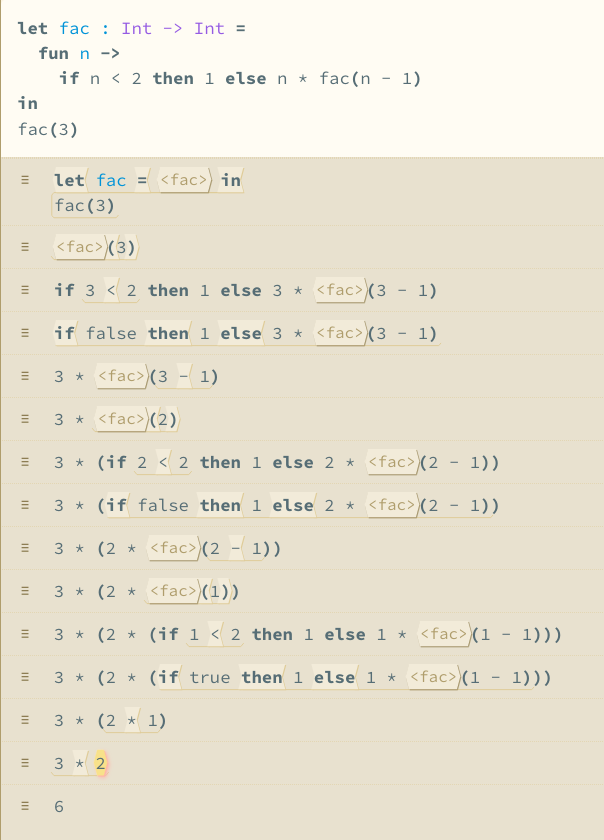
\includegraphics[width=\textwidth]{images/intro-fac-unfiltered.png}}
      \Description{Unfiltered stepper trace for a factorial program, showing many small-step equations from the function definition to the final result 6.}
      \caption{Program trace without filters.}
      \label{fig:intro-fac-unfiltered}
    \end{subfigure}
    \quad
    \begin{subfigure}[t]{0.43\textwidth}
      \centering
      \frame{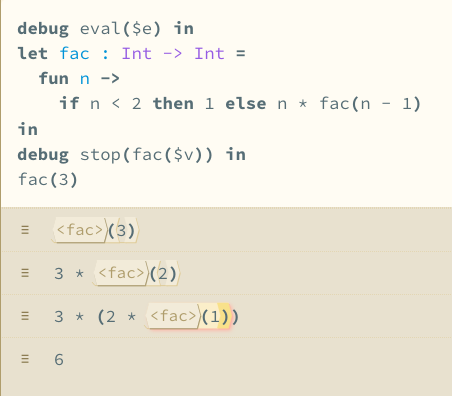
\includegraphics[width=\textwidth]{images/intro-fac-filtered.png}}
      \Description{Filtered stepper trace for the same factorial program, showing only a few key steps and the final result 6.}
      \caption{Program trace with filters that stop at applications of the function to a value.}
      \label{fig:intro-fac-filtered}
    \end{subfigure}
  \end{center}
  \caption{Stepper traces for a factorial program. Filters reduce a long
    sequence of small steps to just the relevant reductions.}
  \label{fig:intro-fac}
\end{figure}

We make the following contributions:
\begin{itemize}
  \item We present the \emph{Filtered Stepper Calculus}, a formal
    semantics for scoped, pattern-based stepping control over
    expression evaluation. We introduce its filter primitives by
    example in Section~\ref{sec:examples}, then formalize the calculus
    in Section~\ref{sec:filter}, where we prove preservation,
    progress, and a simulation theorem (the filtered stepper agrees
    with the underlying unfiltered semantics) and mechanize all proofs
    in Agda.
  \item We implement the filtered stepper in Hazel
    (Section~\ref{sec:implementation}). The implementation reconciles
    Hazel's internal environment-based big-step evaluator with the
    substitution-based presentation expected by students, and includes
    several optimizations to keep interactive stepping responsive.
  \item We deploy the stepper in a university programming languages
    course and report quantitative usage data and survey responses
    from student assignments (Section~\ref{sec:evaluation}).
\end{itemize}

Section~\ref{sec:related} situates the work in related literature, and
Section~\ref{sec:discussion} concludes.

%%% Local Variables:
%%% mode: LaTeX
%%% TeX-master: "main"
%%% End:
